\documentclass[tikz,border=10pt]{standalone}
\usepackage{helvet}
\renewcommand{\familydefault}{\sfdefault}
\usepackage{tikz}
\usetikzlibrary{arrows.meta, positioning, calc, shapes.geometric, decorations.pathreplacing, backgrounds, fit}

\definecolor{emeraldpine}{HTML}{1A4D3E}
\definecolor{harvardcrimson}{HTML}{A51C30}
\definecolor{ethdarkblue}{HTML}{1F407A}
\definecolor{ethpetrol}{HTML}{007A87}
\definecolor{ethbronze}{HTML}{B87333}
\definecolor{ink}{HTML}{1A202C}
\definecolor{cardbg}{HTML}{F8FAFC}
\definecolor{shadecolor}{HTML}{F4F6F9}
\definecolor{paleink}{HTML}{A0AEC0}

\begin{document}
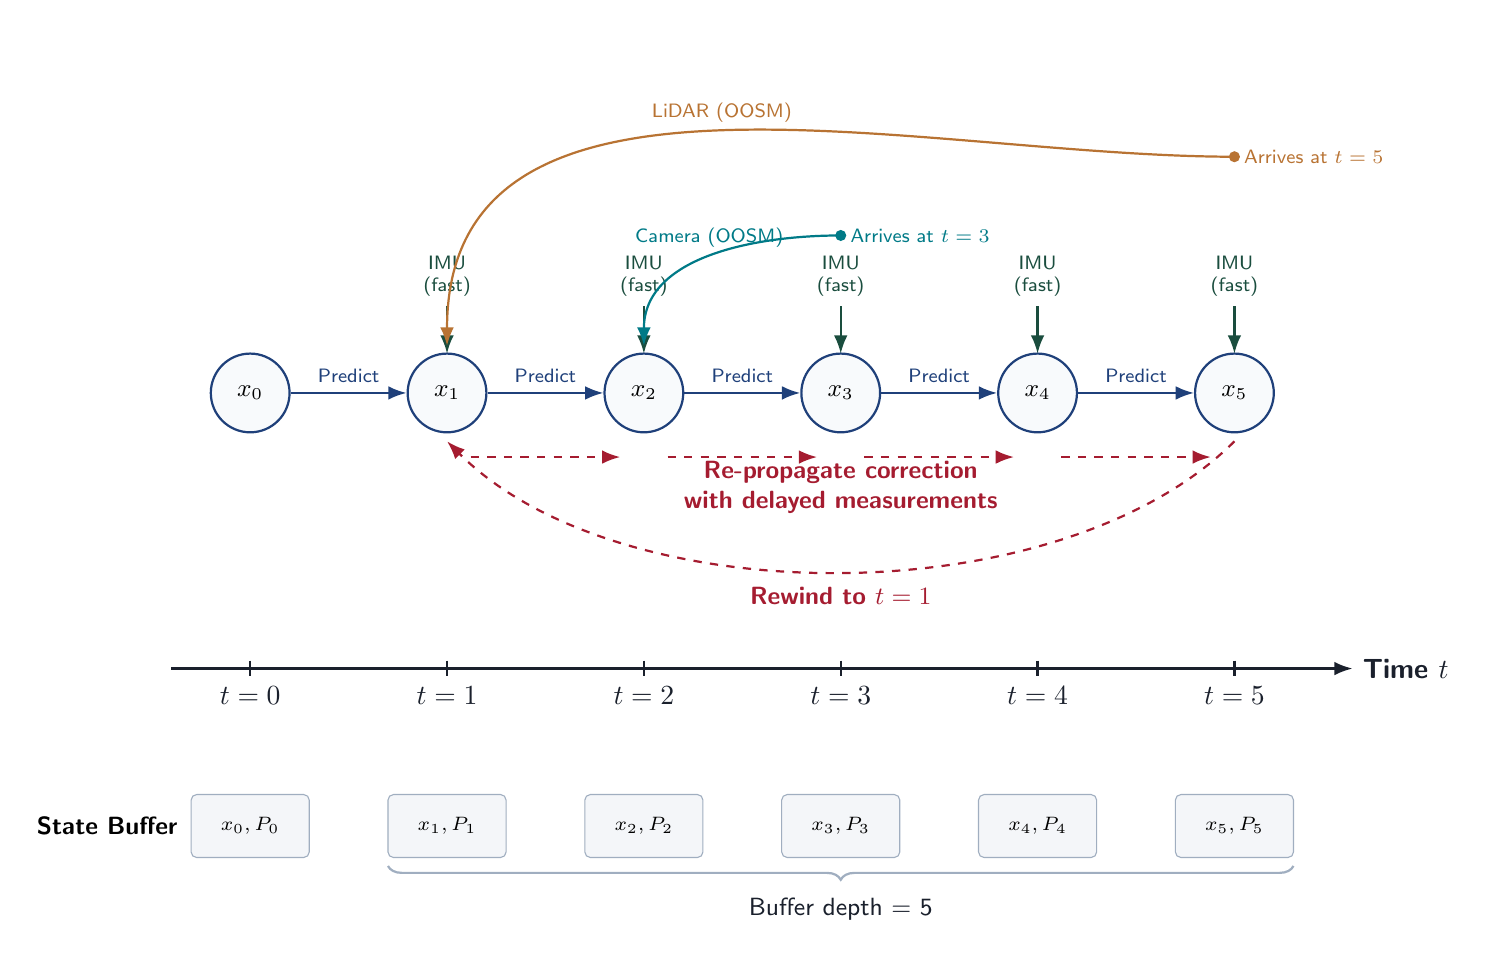
\begin{tikzpicture}[
    >=Latex,
    node distance=2cm,
    font=\sffamily,
    state node/.style={circle, draw=ethdarkblue, fill=cardbg, thick, minimum size=10mm, inner sep=0pt, font=\small\bfseries},
    buffer box/.style={draw=paleink, fill=shadecolor, rounded corners=2pt, minimum width=1.5cm, minimum height=0.8cm, align=center, font=\scriptsize},
]

% Draw timeline (moved to y = -1.0)
\draw[thick, ink, ->] (-1, -1.0) -- (14, -1.0) node[right, font=\bfseries] {Time $t$};
\foreach \t in {0, 1, ..., 5} {
    \draw[thick, ink] (\t*2.5, -0.9) -- (\t*2.5, -1.1) node[below] {$t=\t$};
}

% State nodes (EKF track at y = 2.5)
\foreach \t in {0, 1, ..., 5} {
    \node[state node] (S\t) at (\t*2.5, 2.5) {$x_{\t}$};
}

% Draw EKF state progression
\foreach \t [evaluate=\t as \nextt using int(\t+1)] in {0, 1, ..., 4} {
    \draw[->, thick, ethdarkblue] (S\t) -- (S\nextt) node[midway, above, font=\scriptsize, ethdarkblue] {Predict};
}

% Sensor arrivals
% IMU arrivals (y = 3.6 to 3.0)
\foreach \t in {1, ..., 5} {
    \draw[emeraldpine, thick, ->] (\t*2.5, 3.6) -- (\t*2.5, 3.0) node[pos=0, above, font=\scriptsize, align=center] {IMU\\(fast)};
}

% Camera arrival (t=3 for t=2)
\draw[ethpetrol, thick, ->] (3*2.5, 4.5) to[out=180, in=90] node[above, font=\scriptsize] {Camera (OOSM)} (2*2.5, 3.1);
\fill[ethpetrol] (3*2.5, 4.5) circle (2pt) node[right, font=\scriptsize] {Arrives at $t=3$};

% LiDAR arrival (t=5 for t=1)
\draw[ethbronze, thick, ->] (5*2.5, 5.5) to[out=180, in=90] node[above, font=\scriptsize] {LiDAR (OOSM)} (1*2.5, 3.1);
\fill[ethbronze] (5*2.5, 5.5) circle (2pt) node[right, font=\scriptsize] {Arrives at $t=5$};

% Rewind buffer (moved to y = -3.0)
\node[font=\bfseries\small, anchor=east] at (-0.8, -3.0) {State Buffer};
\foreach \t in {0, 1, ..., 5} {
    \node[buffer box] (B\t) at (\t*2.5, -3.0) {$x_{\t}, P_{\t}$};
}
\draw[decorate, decoration={brace, amplitude=5pt, mirror}, thick, paleink] ([xshift=-0.75cm,yshift=-0.1cm]B1.south) -- ([xshift=0.75cm,yshift=-0.1cm]B5.south) node[midway, below=8pt, font=\small, text=ink] {Buffer depth = 5};

% Rewind action
% LiDAR arrives at t=5, we rewind to t=1
% Curve from S5.south down and back to S1.south
\draw[->, dashed, harvardcrimson, thick] ([yshift=-0.1cm]S5.south) to[out=-135, in=-45, looseness=0.8] node[below=2pt, font=\small\bfseries] {Rewind to $t=1$} ([yshift=-0.1cm]S1.south);

% Repropagation
\foreach \t [evaluate=\t as \nextt using int(\t+1)] in {1, 2, ..., 4} {
    \draw[->, dashed, harvardcrimson, thick] ([xshift=0.3cm, yshift=-0.3cm]S\t.south) -- ([xshift=-0.3cm, yshift=-0.3cm]S\nextt.south);
}

\node[harvardcrimson, font=\small\bfseries, align=center] at (3*2.5, 1.3) {Re-propagate correction\\with delayed measurements};

\end{tikzpicture}
\end{document}
